\documentclass{article}
\usepackage{graphicx}
\usepackage{fullpage}

\begin{document}

\title{LPP: Gameplay \& Namespace (draft)}
\author{Zening Qu}
\maketitle

\section{Gameplay}
We want to produce an RPG game. For that to happen, our game prototype much be rich in (1) user-user interaction (2) user-object interaction. Therefore it is important that we put both kinds of interactions into the gameplay. Here are my proposals for the two types of interactions:

\begin{itemize}
\item User-user Interactions: users send requests to each other; if a request is granted, the requester's experience (figure~\ref{ns}) will grow; such requests could be a drawing of a sheep, but we don't really have to implement them in the front end for now (as long as the request packets are sent out, the gameplay will be able to move on automatically).
\item User-object Interactions: each asteroid maintains a certain number of objects; users interact with these objects to gain experience; such objects could be seedlings that come out of the earth of the asteroid and users should try to get rid of them.
\end{itemize}

\section{Namespace}

\begin{figure}[htbp]
\begin{center}
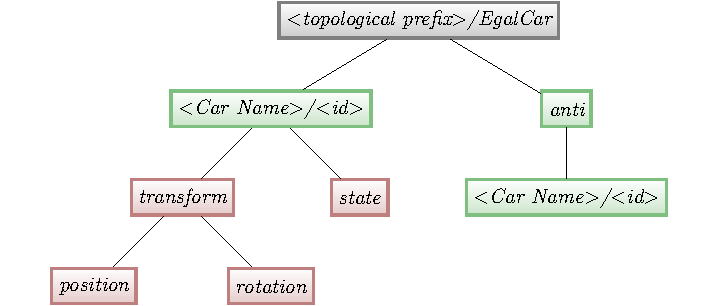
\includegraphics{ObjectTree.pdf}
\caption{Part of LPP's namespace, nodes that contain a ``(sequence number)'' will be explained one by one in this document}
\label{ns}
\end{center}
\end{figure}

\begin{enumerate}
\item \emph{/ndn/ucla.edu/apps/lpp}: the topological prefix of the game
\item \emph{$<$Player ID$>$}: a random number generated in real-time to represent a particular player in the game, this ID is computed in a random manner to (partly) avoid name collisions
\item \emph{$<$Asteroid ID$>$}: a random, real-time number representing a particular asteroid
\item \emph{$<$Seedling ID$>$}: a random, real-time number representing a particular seedling who comes out of a particular asteroid
\item \emph{anti}: this is for asset deletion (publishing an anti-asset corresponds to deleting that particular asset)
\item \emph{.../$<$Player ID$>$/state}: the current state of a particular player; \emph{position} can be used to provide a global view; \emph{experience} can be used to produce a global rank list
\item \emph{.../$<$Asteroid ID$>$/state}: the current state of a particular asteroid, which may contain a name list of all players on that asteroid and things like that
\item \emph{.../$<$Player ID$>$/event}: the action of a particular player
\end{enumerate}

In figure~\ref{ns}, all blue nodes are recognized as \emph{Asset}s, all red nodes \emph{State}s, green ones \emph{Event}s. We will have more documentations about Asset, State, Event in the future. For now it is sufficient to know that these three types of nodes will be synchronized in three different ways.

\end{document}